\documentclass[11pt]{article}\usepackage[]{graphicx}\usepackage[]{color}
% maxwidth is the original width if it is less than linewidth
% otherwise use linewidth (to make sure the graphics do not exceed the margin)
\makeatletter
\def\maxwidth{ %
  \ifdim\Gin@nat@width>\linewidth
    \linewidth
  \else
    \Gin@nat@width
  \fi
}
\makeatother

\definecolor{fgcolor}{rgb}{0.345, 0.345, 0.345}
\newcommand{\hlnum}[1]{\textcolor[rgb]{0.686,0.059,0.569}{#1}}%
\newcommand{\hlstr}[1]{\textcolor[rgb]{0.192,0.494,0.8}{#1}}%
\newcommand{\hlcom}[1]{\textcolor[rgb]{0.678,0.584,0.686}{\textit{#1}}}%
\newcommand{\hlopt}[1]{\textcolor[rgb]{0,0,0}{#1}}%
\newcommand{\hlstd}[1]{\textcolor[rgb]{0.345,0.345,0.345}{#1}}%
\newcommand{\hlkwa}[1]{\textcolor[rgb]{0.161,0.373,0.58}{\textbf{#1}}}%
\newcommand{\hlkwb}[1]{\textcolor[rgb]{0.69,0.353,0.396}{#1}}%
\newcommand{\hlkwc}[1]{\textcolor[rgb]{0.333,0.667,0.333}{#1}}%
\newcommand{\hlkwd}[1]{\textcolor[rgb]{0.737,0.353,0.396}{\textbf{#1}}}%
\let\hlipl\hlkwb

\usepackage{framed}
\makeatletter
\newenvironment{kframe}{%
 \def\at@end@of@kframe{}%
 \ifinner\ifhmode%
  \def\at@end@of@kframe{\end{minipage}}%
  \begin{minipage}{\columnwidth}%
 \fi\fi%
 \def\FrameCommand##1{\hskip\@totalleftmargin \hskip-\fboxsep
 \colorbox{shadecolor}{##1}\hskip-\fboxsep
     % There is no \\@totalrightmargin, so:
     \hskip-\linewidth \hskip-\@totalleftmargin \hskip\columnwidth}%
 \MakeFramed {\advance\hsize-\width
   \@totalleftmargin\z@ \linewidth\hsize
   \@setminipage}}%
 {\par\unskip\endMakeFramed%
 \at@end@of@kframe}
\makeatother

\definecolor{shadecolor}{rgb}{.97, .97, .97}
\definecolor{messagecolor}{rgb}{0, 0, 0}
\definecolor{warningcolor}{rgb}{1, 0, 1}
\definecolor{errorcolor}{rgb}{1, 0, 0}
\newenvironment{knitrout}{}{} % an empty environment to be redefined in TeX

\usepackage{alltt}

\usepackage{rotating}
\usepackage{graphics}
\usepackage{latexsym}
\usepackage{color}
\usepackage{listings}
\usepackage{wrapfig}
\usepackage{float}
\usepackage[belowskip=-15pt,aboveskip=0pt]{caption}

\setlength\topmargin{-.56in}
\setlength\evensidemargin{0in}
\setlength\oddsidemargin{0in}
\setlength\textwidth{6.49in}
\setlength\textheight{8.6in}
\setlength{\intextsep}{10pt plus 1pt minus 4pt}

\definecolor{codegreen}{rgb}{0,0.6,0}
\definecolor{codegray}{rgb}{0.5,0.5,0.5}
\definecolor{codepurple}{rgb}{0.58,0,0.82}
\definecolor{backcolour}{rgb}{0.95,0.95,0.92}
\lstdefinestyle{mystyle}{
	backgroundcolor=\color{backcolour},   
	commentstyle=\color{codegreen},
	keywordstyle=\color{magenta},
	numberstyle=\tiny\color{codegray},
	stringstyle=\color{codepurple},
	basicstyle=\footnotesize,
	breakatwhitespace=false,         
	breaklines=true,                 
	captionpos=b,                    
	keepspaces=true,                 
	numbers=left,                    
	numbersep=5pt,                  
	showspaces=false,                
	showstringspaces=false,
	showtabs=false,                  
	tabsize=2
}
\lstset{style=mystyle}

\pagestyle{headings}

\title{Predictive Model for Average Avocado Prices\vspace{-5ex}} 
\date{December 16, 2020\vspace{-5ex}}
\IfFileExists{upquote.sty}{\usepackage{upquote}}{}
\begin{document} 
\maketitle
\hfill \break
















\noindent\textbf{\underline{Executive Summary}}:      
\hfill \break

\noindent\textbf{\underline{Introduction}}: 
\hfill \break

\noindent\textbf{\underline{Methods}}: 
\hfill \break

\noindent\textbf{\underline{Exploratory Data Analysis}}:  

\begin{figure}[h!] 
\begin{center}

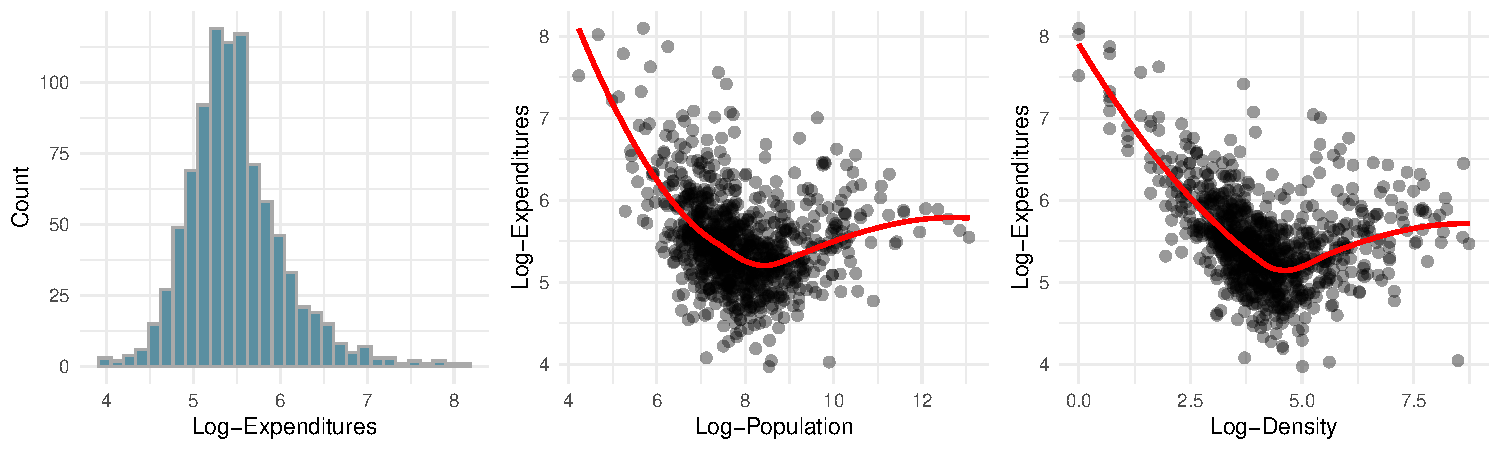
\includegraphics[width=\maxwidth]{figure/unnamed-chunk-1-1} 

\caption{}
\label{explore1}
\end{center} 
\end{figure}


\begin{figure}[h!] 
\begin{center}

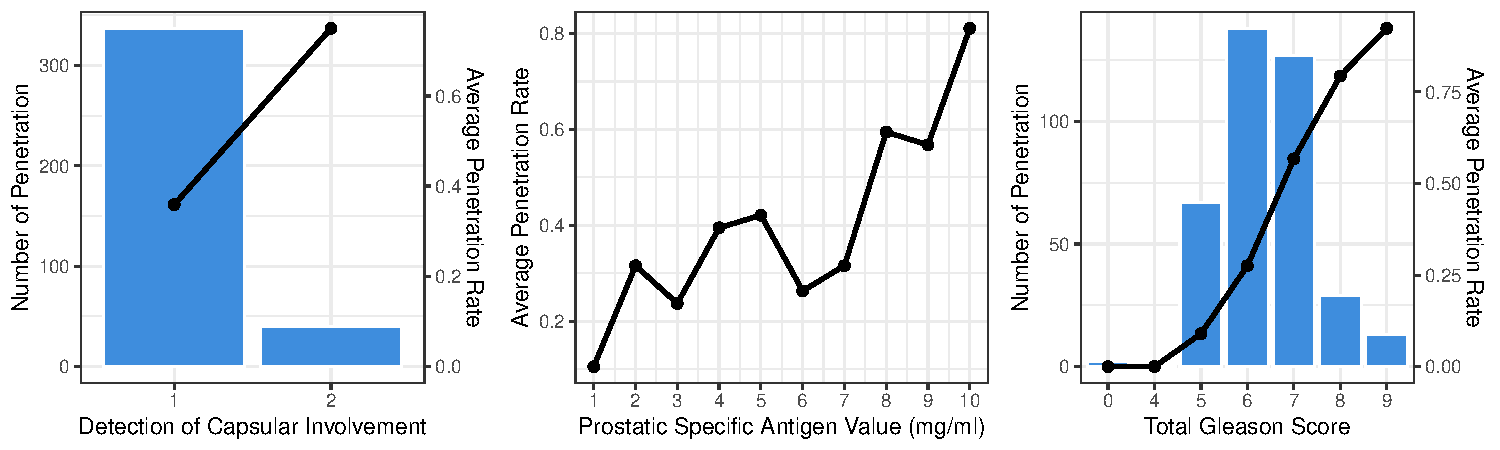
\includegraphics[width=\maxwidth]{figure/unnamed-chunk-2-1} 

\caption{}
\label{explore2}
\end{center} 
\end{figure}


\begin{figure}[h!] 
\begin{center}

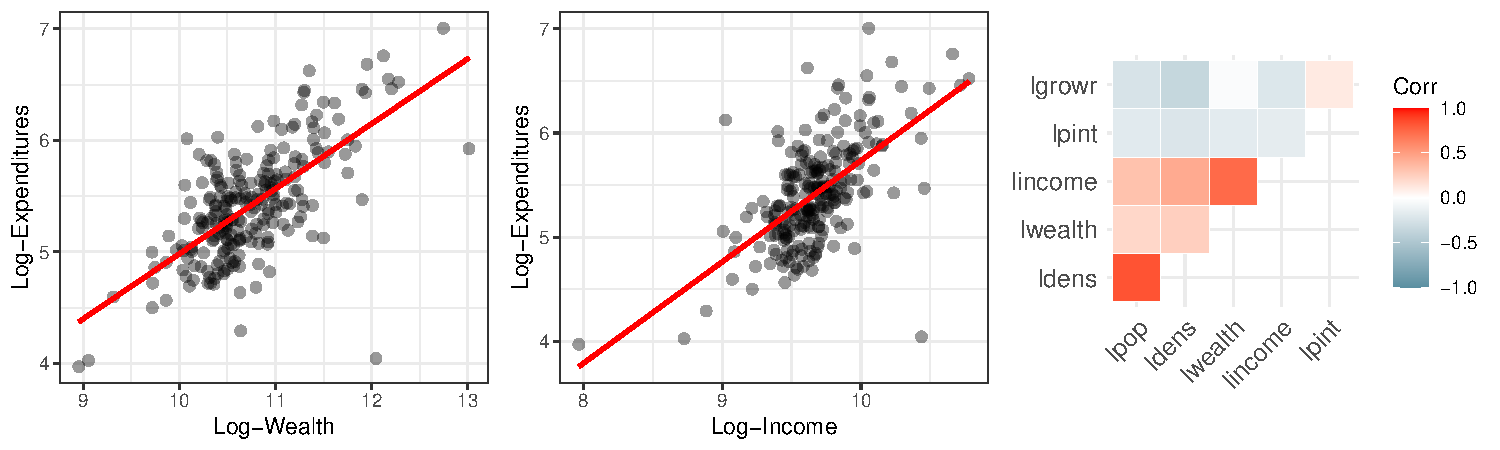
\includegraphics[width=\maxwidth]{figure/unnamed-chunk-3-1} 

\caption{}
\label{explore3}
\end{center} 
\end{figure}





\begin{center}
% latex table generated in R 3.6.2 by xtable 1.8-4 package
% Sun Dec 13 14:49:09 2020
\begin{table}[ht]
\centering
\begin{tabular}{lrrrrrr}
  \hline
Term & Coef & SdError & F-Stat & pValue & 2.5\% CI & 97.5\% CI \\ 
  \hline
(Intercept) & 1.228 & 0.018 & 70.111 & 0.000 & 1.193 & 1.262 \\ 
  log\_total\_volume & -0.029 & 0.001 & -23.237 & 0.000 & -0.031 & -0.026 \\ 
  month2 & -0.037 & 0.008 & -4.712 & 0.000 & -0.052 & -0.021 \\ 
  month3 & 0.031 & 0.008 & 4.066 & 0.000 & 0.016 & 0.045 \\ 
  month4 & 0.094 & 0.008 & 12.402 & 0.000 & 0.079 & 0.109 \\ 
  month5 & 0.080 & 0.008 & 10.502 & 0.000 & 0.065 & 0.095 \\ 
  month6 & 0.134 & 0.008 & 16.547 & 0.000 & 0.118 & 0.149 \\ 
  month7 & 0.198 & 0.008 & 25.137 & 0.000 & 0.182 & 0.213 \\ 
  month8 & 0.223 & 0.008 & 27.667 & 0.000 & 0.207 & 0.239 \\ 
  month9 & 0.242 & 0.008 & 30.527 & 0.000 & 0.227 & 0.258 \\ 
  month10 & 0.192 & 0.008 & 24.207 & 0.000 & 0.176 & 0.207 \\ 
  month11 & 0.113 & 0.008 & 13.961 & 0.000 & 0.097 & 0.129 \\ 
  month12 & 0.026 & 0.008 & 3.202 & 0.001 & 0.010 & 0.043 \\ 
  typeorganic & 0.367 & 0.005 & 67.379 & 0.000 & 0.356 & 0.377 \\ 
  geography\_bins2 & 0.160 & 0.005 & 33.397 & 0.000 & 0.150 & 0.169 \\ 
  geography\_bins3 & 0.309 & 0.005 & 61.764 & 0.000 & 0.299 & 0.318 \\ 
  geography\_bins4 & 0.563 & 0.008 & 69.124 & 0.000 & 0.547 & 0.579 \\ 
   \hline
\end{tabular}
\caption{Summary regression of final model} 
\label{final_fit}
\end{table}

\end{center}








\begin{figure}[h!] 
\begin{center}

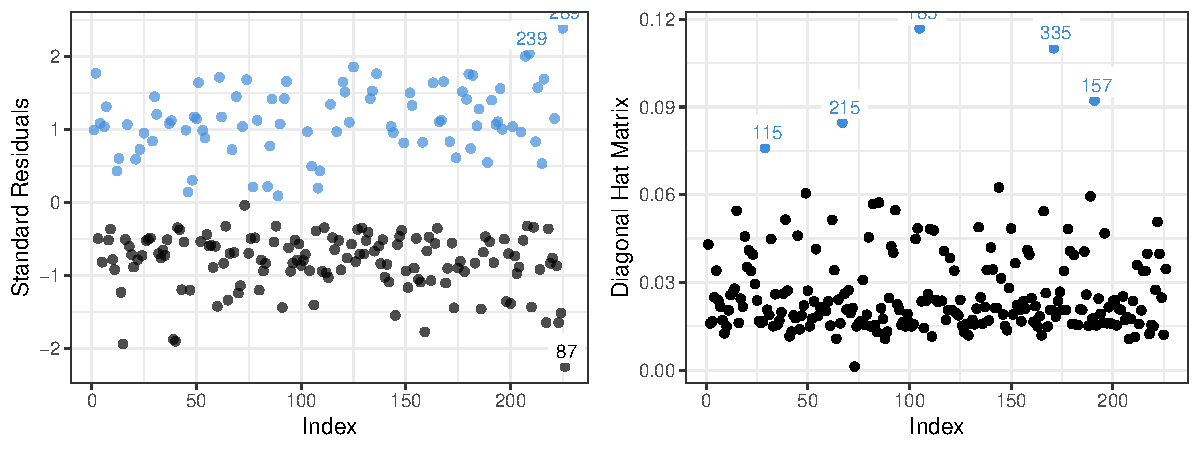
\includegraphics[width=\maxwidth]{figure/unnamed-chunk-5-1} 

\caption{}
\label{explore3}
\end{center} 
\end{figure}


\begin{figure}[h!] 
\begin{center}

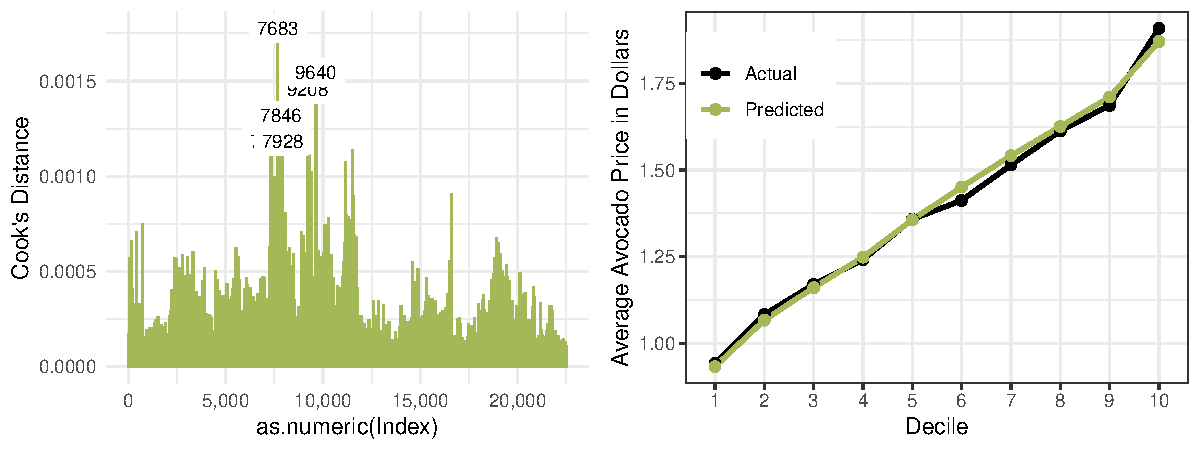
\includegraphics[width=\maxwidth]{figure/unnamed-chunk-6-1} 

\caption{}
\label{explore3}
\end{center} 
\end{figure}


\noindent\textbf{\underline{Model Fitting/Inferences}}: 
\hfill \break

\noindent\textbf{\underline{Conclusion}}: 
\hfill \break

\clearpage
\newpage
\noindent \Large{{\bf Appendix A: Supplemental Tables}}

\begin{center}

% Table created by stargazer v.5.2.2 by Marek Hlavac, Harvard University. E-mail: hlavac at fas.harvard.edu
% Date and time: Sun, Dec 13, 2020 - 2:49:18 PM
\begin{table}[H] \centering 
  \caption{Summary Statistics for all numerical independent features} 
  \label{} 
\begin{tabular}{@{\extracolsep{5pt}}lccccccc} 
\\[-1.8ex]\hline 
\hline \\[-1.8ex] 
Statistic & \multicolumn{1}{c}{N} & \multicolumn{1}{c}{Mean} & \multicolumn{1}{c}{St. Dev.} & \multicolumn{1}{c}{Min} & \multicolumn{1}{c}{Pctl(25)} & \multicolumn{1}{c}{Pctl(75)} & \multicolumn{1}{c}{Max} \\ 
\hline \\[-1.8ex] 
total\_volume & 30,021 & 939,255 & 3,813,519 & 85 & 14,299 & 489,803 & 63,716,144 \\ 
4046 & 30,021 & 299,107 & 1,289,108 & 0 & 783 & 115,156 & 22,743,616 \\ 
4225 & 30,021 & 284,901 & 1,169,078 & 0 & 2,814 & 140,947 & 20,470,573 \\ 
4770 & 30,021 & 21,629 & 100,919 & 0 & 0 & 5,424 & 2,546,439 \\ 
total\_bags & 30,021 & 333,534 & 1,415,618 & 0 & 8,374 & 159,174 & 31,689,189 \\ 
small\_bags & 30,021 & 232,126 & 950,503 & 0 & 5,956 & 112,938 & 20,550,407 \\ 
large\_bags & 30,021 & 95,185 & 467,210 & 0 & 352 & 36,068 & 13,327,601 \\ 
xlarge\_bags & 30,021 & 6,223 & 38,137 & 0 & 0 & 560 & 1,022,564 \\ 
\hline \\[-1.8ex] 
\end{tabular} 
\end{table} 

\end{center}

\begin{center}
% latex table generated in R 3.6.2 by xtable 1.8-4 package
% Sun Dec 13 14:49:19 2020
\begin{table}[ht]
\centering
\begin{tabular}{rp{1.5in}p{.8in}llll}
  \hline
 & Model & Number of Features & MSE & Adj.R.squared & F.statistics & AIC \\ 
  \hline
1 & Initial Model & 16.000 & 0.062 & 0.572 & 1879.873 & 1421.841 \\ 
  2 & Stepwise Model & 16.000 & 0.062 & 0.572 & 1879.873 & 1421.841 \\ 
  3 & Model with Interaction Terms & 78.000 & 0.060 & 0.588 & 413.437 & 598.507 \\ 
  4 & Stepwise Model with Interaction Terms & 77.000 & 0.060 & 0.588 & 418.808 & 597.053 \\ 
   \hline
\end{tabular}
\caption{Regression validation metrics including MSE, R-squared adjusted, and AIC} 
\label{reg_vali_metric}
\end{table}

\end{center} 


\begin{center}
% latex table generated in R 3.6.2 by xtable 1.8-4 package
% Sun Dec 13 14:49:19 2020
\begin{table}[ht]
\centering
\begin{tabular}{rrrr}
  \hline
 & GVIF & Df & GVIF\verb|^|(1/(2*Df)) \\ 
  \hline
log\_total\_volume & 2.713 & 1.000 & 1.647 \\ 
  month & 1.007 & 11.000 & 1.000 \\ 
  type & 2.673 & 1.000 & 1.635 \\ 
  geography\_bins & 1.031 & 3.000 & 1.005 \\ 
   \hline
\end{tabular}
\caption{} 
\label{vif_table}
\end{table}

\end{center} 

\clearpage
\newpage
\noindent \Large{{\bf Appendix B: R Code}}
\lstinputlisting[language=R, caption = Appendix of Code]{R/dar3-codes.R}


\end{document}






